\chapter{Esempio}
    Si sceglie come esempio \cite{kouWearableAllFabricHybrid2024}, che offre una realizzazione pratica di un harvester ibrido. L'obbiettivo di questo generatore \'e proporre un dispositivo riproducibile in scala e facilmente integrabile nel vestiario. Per fare questo usa una struttura interamente fondata su una base di tessuto e accoppia un generatore triboelettrico a uno RF. Un tessuto elettricamente conduttivo disponibile sul mercato \'e usato per realizzare le connessioni su ambo i lati di uno strato di tessuto comune di cotone. In questo modo l'harvester diventa altamente flessibile e facilmente integrabile in capi di abbigliamento. Viene poi proposto un metodo efficace per la produzione di dispositivi elettronici basati su tessuto. Avere 2 fonti energetiche distinte aumenta le probabilit\'a che il dispositivo sia sempre in funzione, inoltre queste in particolare si prestano a un design planare.
    
    \begin{figure}[H]
        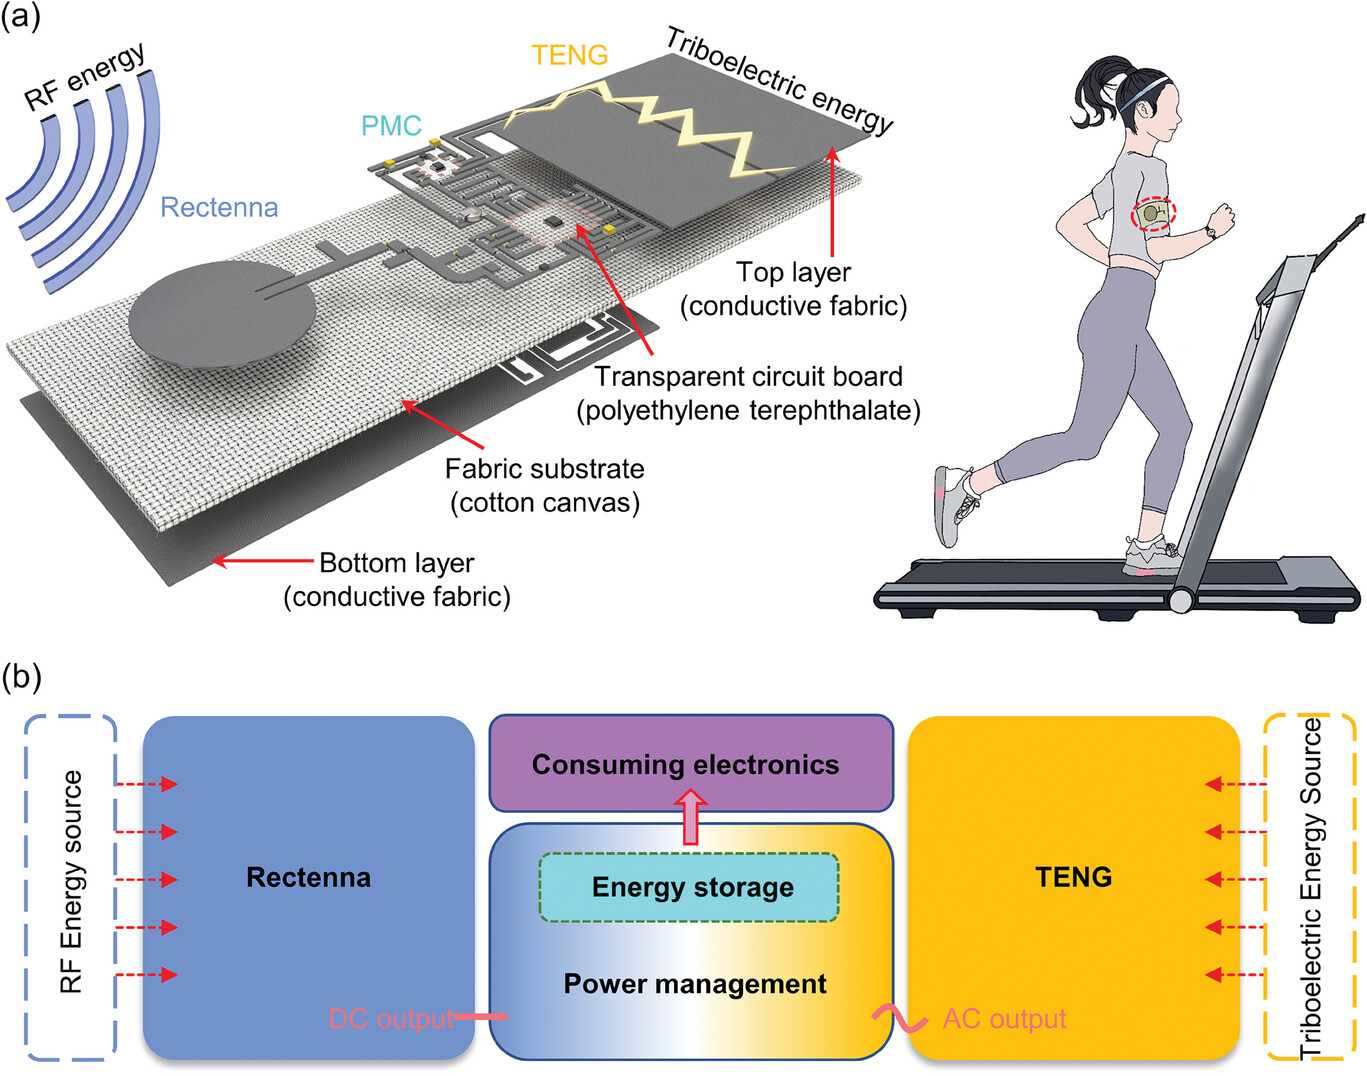
\includegraphics[width=0.7\textwidth]{schema.jpg}
        \centering
        \caption{a) Modello della struttura dell'harvester preso in esempio. b) Schema del funzionamento generale dell'harvester.\cite{kouWearableAllFabricHybrid2024}}
        \label{fig:schema}
    \end{figure}

\begin{section}{Generatori}
    \begin{subsection}{Generatore Triboelettrico}
        In generale i generatori di questo tipo sfruttano la capacit\'a di alcuni materiali di trasferire carica al contatto o sfregamento. La struttura \'e formata da uno strato di propilene fluorato (FEP) libero di scorrere sopra ai due elettrodi di tessuto connettivo che doppiano da secondo materiale triboelettrico. Questa forma, detta a scorrimento libero, oltre ad avere un fattore di forma pi\'u vantaggioso, genera anche pi\'u energia rispetto al semplice contatto \cite{fuAchievingUltraDurabilityHigh2024}. 
        \begin{figure}[H]
            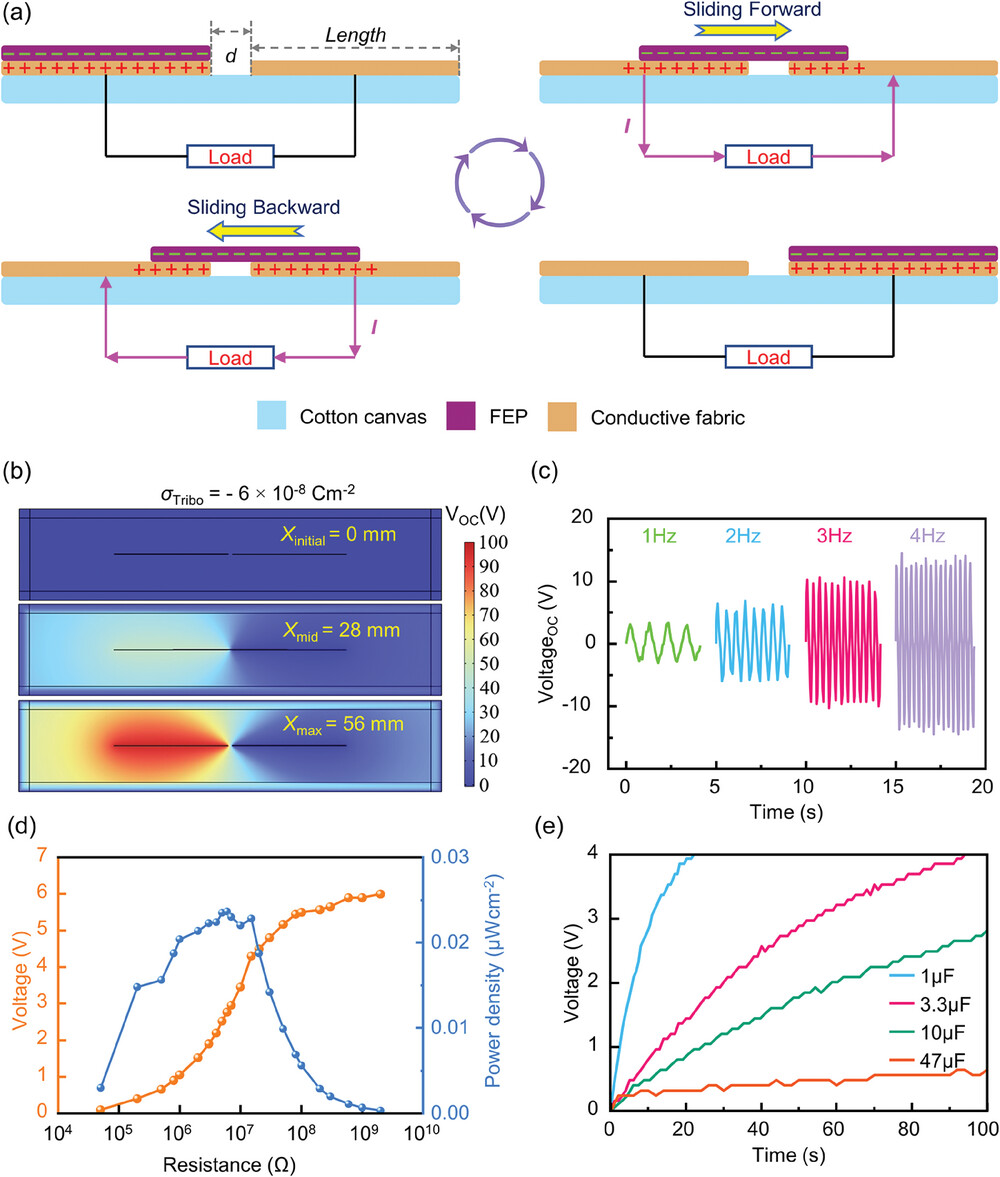
\includegraphics[width=0.8\textwidth]{funzioneTEG.jpg}
            \centering
            \caption{a) Schema del funzionamento del generatore triboelettrico. b) Potenziali simulati a spostamento iniziale, medio e massimo. c) Uscita in tensione a diverse frequenze di scorrimento. d) Dipendenza della tensione e potenza prodotte dal carico. e) Tempi di carica di condensatori commerciali.\cite{kouWearableAllFabricHybrid2024}}
            \label{fig:funzioneTEG}
        \end{figure}
        Il design aperto e i limiti di peso non permettono di ottimizzare altri aspetti che influenzano l'efficienza, come l'umidit\'a o la pressione tra gli elementi. La tensione massima ottenibile tra gli elettrodi \'e determinata dalla densit\'a di carica prodotta dal contatto dei materiali. Lo stimolo meccanico genera nello strato libero un movimento oscillatorio e quindi una corrente alternata sul circuito, necessita perci\'o di raddrizzamento. La densit\'a di potenza massima \(0.024\mu Wcm^{-2}\), \'e stata misurata collegando un potenziometro e azionando il movimento a \(2Hz\) per simulare il cammino. Per quanto questo dimostri che il dispositivo \'e in grado di raccogliere energia dal movimento umano, la densit\'a di potenza \'e molto bassa se paragonata a una batteria tradizionale, ma anche ai requisiti correnti di dispositivi medici indossabili \cite{gaoAdvancedEnergyHarvesters2024}. Il funzionamento e i risultati sperimentali sono raccolti in figura \ref{fig:funzioneTEG}.
        
    \end{subsection}
    
    \begin{subsection}{Generatore a Radiofrequenza}
        Per raccogliere energia dalle radiazioni presenti nell'ambiente, \'e stato scelto un harvester con antenna dimensionata per la sola banda attorno ai \(2.45GHz\), usata per connessioni a corto raggio come Wi-Fi e Bluetooth. La distribuzione di onde radio dovute alle comunicazioni elettroniche \'e naturalmente concentrata nelle zone urbane. In aree extraurbane la densit\'a di potenza dovuta a comunicazioni ad ampio raggio scende vistosamente \cite{ibrahimRadioFrequencyEnergy2022}, la scelta di una banda comunemente usata da dispositivi generalmente vicini all'uomo ha quindi il vantaggio di essere pi\'u consistente nel tempo. La configurazione per l'antenna \'e a patch circolare e le dimensioni ottimali per la risonanza sono stati ottenuti attraverso simulazione. Il valore di specific absorbtion rate (SAR) \'e un parametro usato per determinare la potenza assorbita da un'unit\'a di massa di tessuto corporeo \cite{vallozzi26LatestDevelopments2016}. Secondo le simulazioni il SAR \'e \(0.073\frac{W}{Kg}\), ben inferiore ai \(2.0\frac{W}{Kg}\) stabiliti dalle norme europee per antenne mobili. In questo caso il SAR \'e usato come parametro di efficienza rispetto alla quantit\'a di radiazione persa dall'antenna nel corpo. 


        
        Un analizzatore (Keysight N5227B) \'e usato per misurare la return loss (RL) in condizioni libera e a contatto col corpo. 
        La return loss \'e definita come:
        \begin{equation*}
            \begin{aligned}
            RL&=10\log_{10}\left( \frac{P_{in}}{P_{ref}} \right) \mathrm{dB}\\
            RL&=-S_{11}
            \end{aligned}
        \end{equation*}
        Dove \(S_{11}\) \'e uno dei parametri di scattering misurati dall'analizzatore, graficato in figura \ref{fig:funzioneRF}. Per le dimensioni scelte si nota effettivamente un picco di \(10\mathrm{dB}\) nel centro banda desiderato. Anche quando l'antenna \'e indossata, lo stesso picco trasla di solo \(20\mathrm{MHz}\).
        

        \begin{figure}[hbt!]
            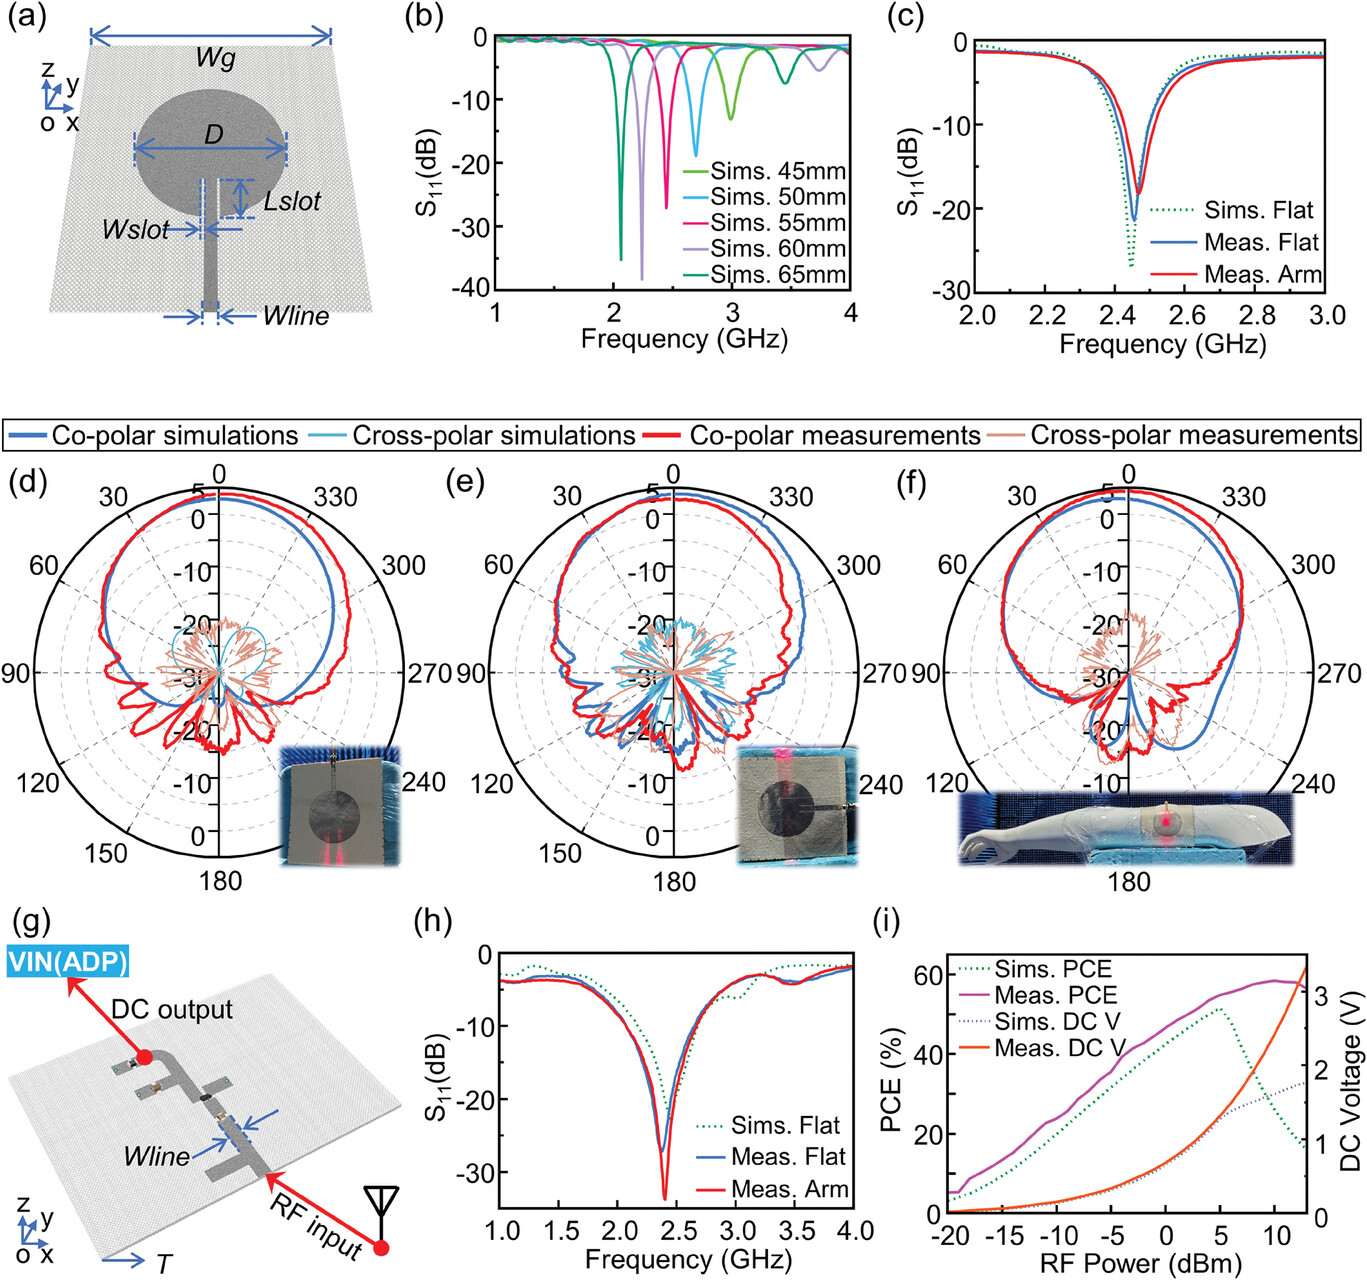
\includegraphics[width=0.8\textwidth]{funzioneRF.jpg}
            \centering
            \caption{a) Struttura dell'antenna. b) Return loss simulata con diversi diametri. c) Return loss misurata con antenna piatta e attaccata al corpo. d) Schema di radiazione con antenna piatta sul piano xoz. e) Schema di radiazione con antenna piatta sul piano xoy. f) Schema di radiazione con antenna flessa sul piano xoz. g) Schema della struttura del raddrizzatore. h) Misure e simulazione della return loss quando l'antenna \'e piatta o attaccata a un braccio. i) Corrente DC ed efficienza di conversione della potenza misurata e simulata rispetto alla potenza in ingresso.\cite{kouWearableAllFabricHybrid2024}}
            \label{fig:funzioneRF}
        \end{figure}
        
        Usando una camera anecoica per microonde \'e stato graficato lo schema di radiazione in varie posizioni. Lo schema bidimensionale segue le curve dove il guadagno del dispositivo \'e massimo. A causa della configurazione della camera di prova \'e stato necessario montare l'antenna su un modello di braccio per caratterizzarne la funzione in flessione. Le misure sono in accordo con le simulazioni e non si presentano particolari differenze nei lobi dovute al cambio di inclinazione o flessione. Quindi si pu\'o dire che l'antenna \'e adatta al funzionamento quando indossata, anche se in posizioni piane come petto e dorso, ma anche dove \'e soggetta alla curvatura come in gambe e braccia.

        Un circuito di raddrizzamento per la corrente in uscita dall'antenna \'e strettamente necessario per poi caricare la batteria. Il raddrizzatore \'e stato progettato per soddisfare alcuni requisiti essenziali. Deve essere flessibile abbastanza da risultare comodamente indossabile. Deve avere massima efficienza di conversione nelle condizioni previste. In fine, \'e necessario che le linee conduttive siano dimensionate con precisione, sia la lunghezza che la larghezza influiscono sul buon accoppiamento all'impedenza dell'antenna. Le microstrip di tessuto conduttivo sono tutte larghe \(4.4\mathrm{mm}\), cos\'i come la linea in uscita dall'antenna. Si fa uso di un raddrizzatore a doppia semionda, con topologia di Greinacher per amplificare la tensione prodotta. Vengono installati due condensatori da \(100\mathrm{pF}\) e due diodi SMS7630-005FL di tipo Schottky, che hanno migliori prestazioni ad alta frequenza e perdite pi\'u basse rispetto ai diodi a giunzione. 

        \begin{figure}[H]
            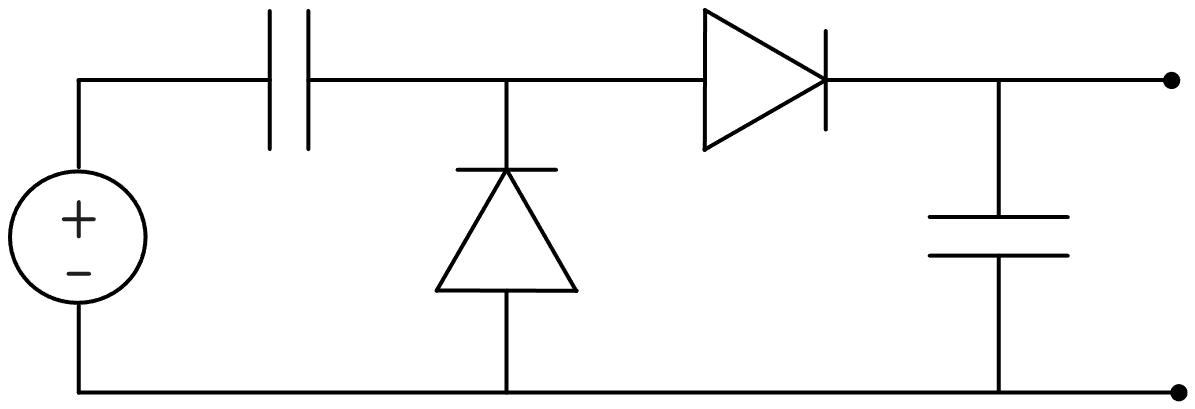
\includegraphics[width=0.6\textwidth]{Greinacher.png}
            \centering
            \caption{Raddrizzatore e amplificatore Greinacher al primo ordine.}
            \label{fig:Greinacher}
        \end{figure}
        
        Nel circuito raddrizzatore per il generatore triboelettrico, integrato in un chip, sono stati scelti invece dei diodi pi\'u efficaci a basse frequenze. Separando il raddrizzatore dal PMC (power management circuit), la coppia antenna/raddrizzatore diventa un modulo facilmente integrabile in altri dispositivi. La capacit\'a del modulo di convertire una potenza in ingresso sotto forma RF in DC \'e stata valutata inserendo un resistore da \(1\mathrm{K\Omega}\) come carico. La fonte RF \'e stata creata usando un generatore di onde (SG-3000PRO) a vari livelli di potenza. L'efficienza di conversione in potenza \'e stata determinata misurando la tensione ai capi del carico.
        \begin{equation*}
            PCE = \frac{P_{carico}}{P_{RF}} = \frac{V_{carico}}{R_{carico}^2P_{RF}}
        \end{equation*}
        I risultati sono graficati in figura \ref{fig:funzioneRF} e mostrano un picco del \(58\%\) nell'efficienza di conversione con \(10\mathrm{dBmW}\) in ingresso, che \'e un valore comune nell'intervallo di potenze usate nelle comunicazioni wireless tra dispositivi mobili. 
    \end{subsection}
\end{section}

\begin{section}{Integrazione}
    I due generatori hanno impedenze diverse in uscita, i moduli sono infatti tre ordini di grandezza distanti. Non possono quindi alimentare direttamente la stessa interfaccia se si vuole alto rendimento. Si sviluppa un PMC per convogliare l'energia prodotta dai due in una singola batteria. Il PMC in questo caso deve svolgere le funzioni di: maximum power point tracking (MPPT), undervoltage lockout (UVLO) e protezione di carica. Due circuiti integrati (ADP5091 e LTC3588), configurati come in figura \ref{fig:schemaPMC}, gestiscono tutte le funzioni. Sono entrambi progettati per applicazioni a bassa potenza e non richiedono alimentazione oltre quella prodotta dall'harvester stesso. Il ADP5091 \'e usato per gestire l'output del generatore RF e proteggere la batteria. In particolare l'uscita REG\_OUT dell'ADP offre la tensione di uscita per il dispositivo da collegare all'harvester quando il componente di accumulo ha raggiunto la tensione minima. Il LTC3588 \'e usato per gestire l'output del generatore triboelettrico. Un raddrizzatore ad alta efficienza per alte frequenze \'e integrato  tra i pin di ingresso, questo funziona anche da blocco per flussi di corrente verso il TEG.

    \begin{figure}[hbt!]
        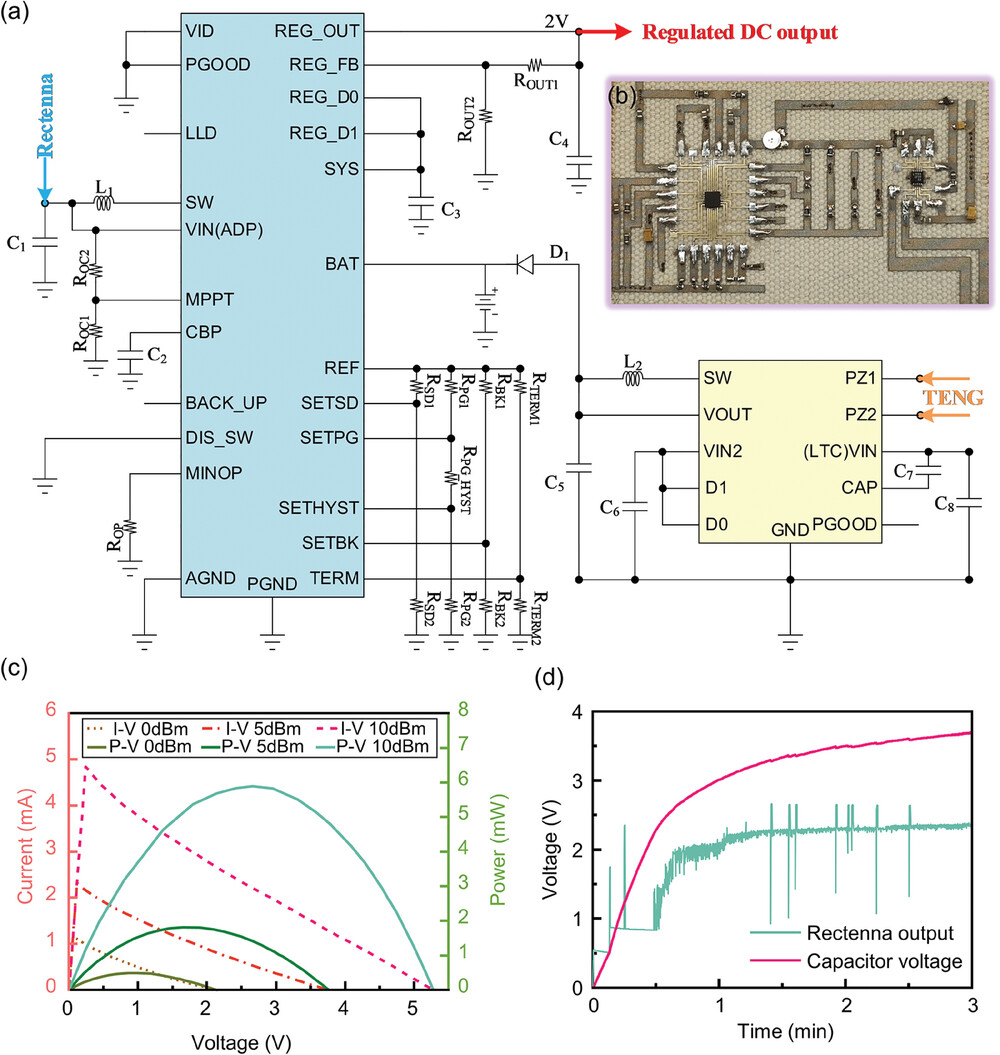
\includegraphics[width=0.9\textwidth]{schemaPMC.jpg}
        \centering
        \caption{a) Schema circuitale del PMC. b) Vista dall'alto del PMC assemblato sul tessuto. c) Dipendenza di corrente e potenza dalla tensione all'uscita del raddrizzatore, per diversi livelli di potenza in ingresso. d) Crescita del potenziale misurata in fase di carica.\cite{kouWearableAllFabricHybrid2024}}
        \label{fig:schemaPMC}
    \end{figure}

    \begin{subsection}{MPPT}
        Le tecniche di MPPT cercano di ottimizzare la potenza convertita da un generatore modificando l'impedenza del circuito, in modo da ottenere il massimo prodotto tra tensione e corrente. Il metodo di MPPT \'e fractional open circuit voltage (FOCV), come descritto nel datasheet del ADP5091 \cite{ADP5091DatasheetProduct}. Il metodo FOCV \'e comunemente usato in campo fotovoltaico, ma il funzionamento del modulo antenna e raddrizzatore \'e paragonabile. L'uscita in tensione varia poco all'interno della banda di frequenze interessata, ma varia considerevolmente con l'incidenza delle onde. La tensione in condizione di circuito aperto varia al variare dell'incidenza di onde RF, la MCU ne prende periodicamente un campione, salvandola in un condensatore. La tensione di massima potenza \'e calcolata secondo:
        \begin{equation*}
            V_{MPPT} = V_{IN}\underbrace{\left(\frac{R_{OC1}}{R_{OC1}+R_{OC2}}\right)}_\mathrm{k}
         \end{equation*}
        Il processore cambia poi l'impedenza di ingresso alla porta VIN a cui \'e collegato il raddrizzatore in modo da ottenere la tensione ottimale. Il fattore moltiplicativo dato dalle resistenze \'e stato determinato sperimentalmente usando una resistenza programmabile mentre l'harvester era sottoposto a diversi livelli di irradiazione (\(0\mathrm{dBmW},5\mathrm{dBmW},10\mathrm{dBmW}\)). Il valore medio del fattore moltiplicativo \'e \(0.5\), per cui sono stati installati due resistori \((R_{OC1},R_{OC2})\) uguali da \(10\mathrm{M\Omega}\). Il periodo di campionamento di default \'e \(16\mathrm{s}\), mentre il tempo per il campionamento \'e \(256\mathrm{ms}\), nessuno dei due \'e stato modificato.
    \end{subsection}

    \begin{subsection}{UVLO}
        L'UVLO \'e implementato nel controllore LTC3588, che gestisce la produzione del generatore triboelettrico. Un condensatore \((C_8)\) immagazzina preventivamente l'energia in entrata. Quando la tensione su  \(C_8\) supera la soglia scelta per UVLO, viene stabilita una connessione attraverso un convertitore di tensione step-down per caricare \(C_5\). Quest'ultimo condensatore \'e collegato alla batteria, e la sua corrente \'e direzionata da un diodo. Sia in ingresso che uscita sono stati usati condensatori elettrolitici al tantalio, per via della migliore capacit\'a, efficienza di carica e bassa corrente di dispersione \cite{torkiElectrolyticCapacitorProperties2023}.
    \end{subsection}

    \begin{subsection}{Protezione di Carica}
        Mantenere la tensione imposta sulla batteria all'interno di un certo intervallo \'e essenziale per ridurne l'usura. La carica massima \'e stabilita a \(3.6\mathrm{V}\) attraverso il dimensionamento delle resistenze \(R_{TERM1}=5.9\mathrm{M\Omega},R_{TERM2}=4.12\mathrm{M\Omega}\), la somma delle resistenze \'e sopra ai \(6\mathrm{M\Omega}\), come consigliato dal produttore del MCU per limitare la corrente di quiescenza. La relazione che determina la tensione massima ammessa \'e:
        \begin{equation*}
            V_{BAT\_TERM} = \frac{3}{2}V_{INT\_REF}\left(1+\frac{R_{TERM1}}{R_{TERM2}}\right) \approx 3.6V
        \end{equation*}
        Dove \(V_{INT\_REF}=1.011\mathrm{V}\), \'e la tensione di riferimento generata internamente.
        %anche scarica valori in S
    \end{subsection}

    \begin{subsection}{Integrazione}
        L'harvester ibrido \'e stato testato in condizioni controllate, misurando quanto velocemente carica un supercondesatore da \(1000\mathrm{\mu F}\). La fonte RF \'e stata posta a \(12\mathrm{cm}\) e emette \(13\mathrm{dBmW}\), mentre il movimento \'e azionato da un attuatore lineare a \(2\mathrm{Hz}\). In queste condizioni il condensatore supera di poco la tensione massima stabilita e resta stabile a \(3.7\mathrm{V}\) dopo \(3\mathrm{m}\). Si ottiene una potenza media di \(38\mathrm{\mu W}\), con picco \(111\mathrm{\mu W}\), che alle dimensioni di \(10\mathrm{cm}\times30\mathrm{cm}\) corrisponde a \(0.13\mathrm{ \frac{\mu W}{cm^2}}\) medi. Per verificarne l'applicabilit\'a a un caso pratico, l'harvester con condensatore carico \'e stato indossato da un volontario e collegato a due dispositivi di cui \'e stato misurato il tempo di funzionamento. Un sensore di temperatura commerciale ha portato il condensatore da \(3.65\mathrm{V}\) alla sua tensione di funzionamento minima \(1.5\mathrm{V}\) in \(42\mathrm{s}\). Un orologio meccanico con tensione operativa di \(1\mathrm{V}\) funziona invece fino a \(32\mathrm{m}\).
        I tempi di carica dei generatori singoli e la modalit\'a ibrida sono stati raccolti in un grafico in figura \ref{fig:risultati}. Da qui si pu\'o notare come la potenza generata dalla parte triboelettrica sia trascurabile rispetto a quella generata dall'antenna.
        \begin{figure}{H}
            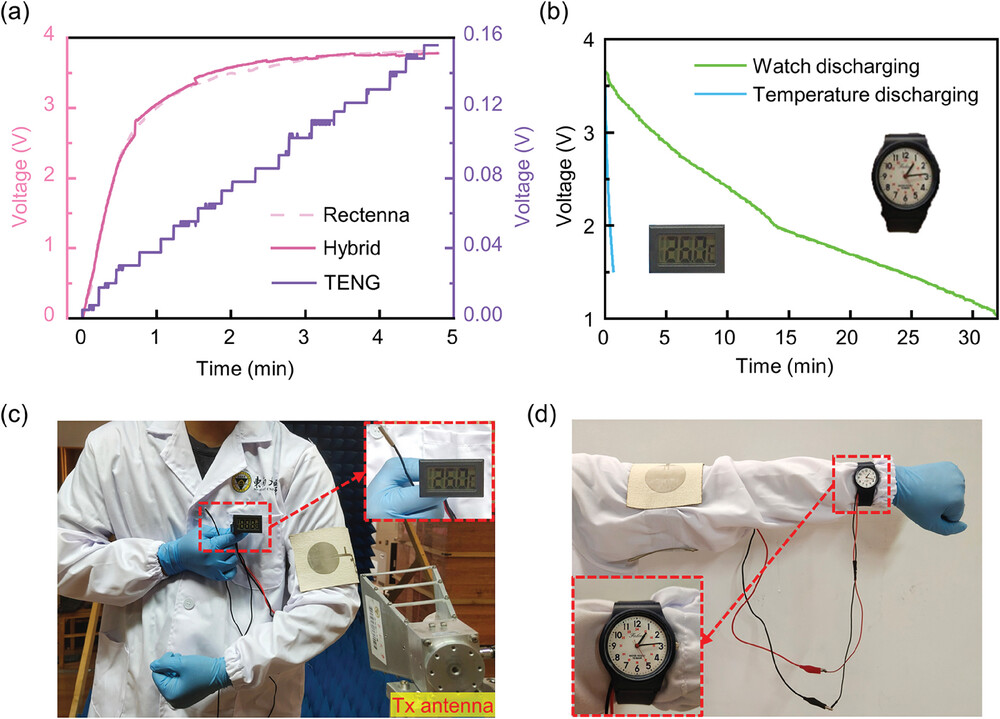
\includegraphics[width=0.85\textwidth]{risultati.jpg}
            \centering
            \caption{a) Tempi di carica singoli e modalit\'a ibrida. b) Tempi di funzionamento dispositivi reali. c) Configurazione sensore di temperatura. d) Configurazione orologio. \cite{kouWearableAllFabricHybrid2024}}
            \label{fig:risultati}
        \end{figure}
        L'inefficienza del generatore triboelettrico causa una caduta considerevole nella densit\'a di potenza generata dall'harvester. Avere una seconda fonte energetica \'e comunque utile quando dovesse mancare l'accesso a sorgenti wireless. Inoltre, il dispositivo con base di tessuto \'e destinato a uso esterno e facilmente integrabile nel vestiario, pu\'o quindi permettersi di essere esteso per aumentare la potenza totale prodotta. Si potrebbero per\'o considerare fonti alternative come fotovoltaico o termoelettrico, che nella stessa posizione non si trovano in condizioni di bassa efficienza come il triboelettrico. Rispetto a queste, i vantaggi sono certamente il costo e la facilit\'a della produzione del generatore triboelettrico.
    \end{subsection}

    %potrei guardare simulazioni o produzione su tessuto


\end{section}